\documentclass[oneside]{UOIT_Thesis}

\usepackage{lipsum} % Only for the sample

\title{Your Thesis Title}
\date{\today}
\author{Your Name}
\degree{Your Degree}
\faculty{Your Faculty}
\program{Your Program}
% By default the university is UOIT, this can be changed by uncommenting the following 
%\university{Your University}

\begin{document}
\pagenumbering{roman} 
\maketitle

\makeabstract{
Put your abstract here.
}

\makeacknowledgements{
Thank some people that you like here.
}

\makedeclaration

{\hypersetup{linkcolor=black}
\maketableofcontents
}

\pagenumbering{arabic}
\doublespacing

\chapter{First Chapter Title}
\lipsum[1-2]
\section{First Section}
\lipsum[3-4]

\chapter{Second Chapter Title}
\lipsum[5-6]
\begin{figure}[tbp]
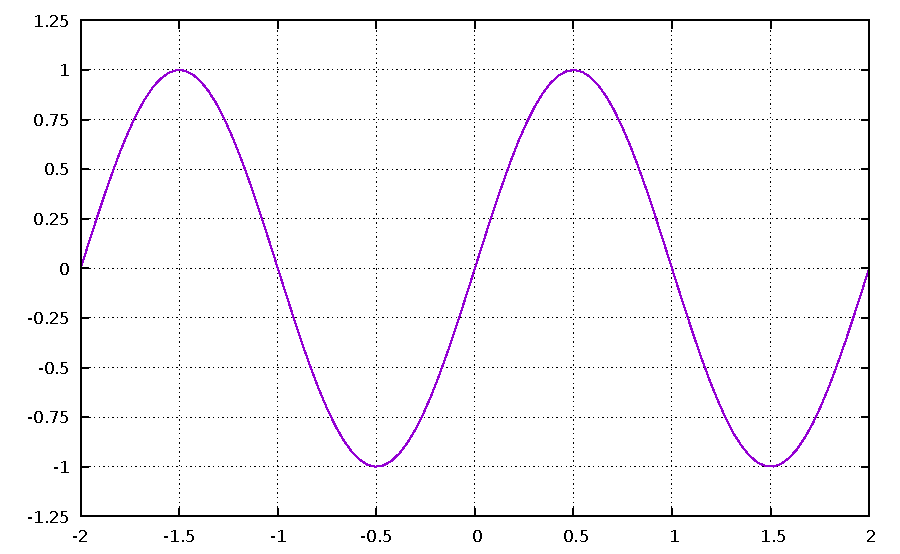
\includegraphics{Plot}
\caption{Beautiful plot of $y = \sin(\pi x)$.}
\end{figure}
\lipsum[7-8]

% Adds references to table of contents
\phantomsection 
\addcontentsline{toc}{chapter}{References} 

\nocite{*} % Only for the sample
\bibliography{Ref}

\appendix

\chapter{Sample Appendix}
\lipsum[9-12]

\end{document}
